\newpage

% question six
\question{6}{0.9 points}

\subquestion{a}{Reflect on the interpretation of the BMI coefficient. Does it capture the \textbf{causal effect} of body fat on income?}

The BMI coefficient reflects the relation between BMI and income; however, it does not capture the causal effect of body fat on income. This means that we cannot confidently establish causality between the two variables by looking at the regression alone. Many scenarios, such as reverse causality, bidirectional causality or even no true causal relationship confounded by omitted variables could explain the coefficient estimated by our model (which is, worth noting, not statistically significant in the regression models discussed so far).

\subquestion{b}{Draw a \textbf{DAG} illustrating how an \textbf{omitted variable} could bias the estimated effect of BMI on income and indicate one such variable.}

A possible omitted variable would be educational attainment, due to its strong effect on both income and BMI. Higher education could likely be positively correlated to income and, through factors such as health knowledge, organizational skills and discipline, negatively correlated to BMI scores. The following DAG illustrates this dynamic:

\begin{figure}[H]
    \centering
    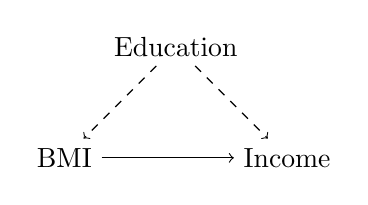
\begin{tikzpicture}[node distance=2cm]
        \node (edu) {Education};
        \node (bmi) [below left of=edu] {BMI};
        \node (inc) [below right of=edu] {Income};

        \draw[dashed, ->] (edu) -- (bmi);
        \draw[dashed, ->] (edu) -- (inc);
        \draw[->] (bmi) -- (inc);
    \end{tikzpicture}
    \caption{DAG showing omitted variable bias}
    \label{fig:dag}
\end{figure}

\subquestion{c}{Based on your DAG, would the resulting bias in the BMI coefficient be \textbf{upward or downward}? Explain.}

Since Education would likely be positively correlated to the dependent variable Income and negatively correlated to the explicative variable BMI, we would expect a model that omits education to be biased towards showing a negative relationship between income and BMI, even if the true effect were to be neutral or positive. In our model, the BMI variables have been trying to account for both their own effect and the effect of education on income.

\newpage

\subquestion{d}{Identify a variable (not necessarily observed in your dataset) that could act as a \textbf{collider} in this context. Use a DAG to illustrate and explain why conditioning on it would lead to bias.}

A collider variable is a variable caused by both the dependent and explicative variables. In the case of our model, a collider variable could be Health Insurance, since both higher BMI and lower income are likely correlated to worse health coverage. A simple DAG illustrating this effect would look as follows:

\begin{figure}[H]
    \centering
    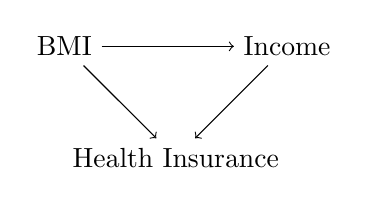
\begin{tikzpicture}[node distance=2cm]
        \node (ins) {Health Insurance};
        \node (bmi) [above left of=ins] {BMI};
        \node (inc) [above right of=ins] {Income};
        
        \draw[->] (inc) -- (ins);
        \draw[->] (bmi) -- (ins);
        \draw[->] (bmi) -- (inc);
    \end{tikzpicture}
    \caption{DAG showing Health Insurance as a collider}
    \label{fig:collider}
\end{figure}